\documentclass[11pt,]{article}
\usepackage{lmodern}
\usepackage{amssymb,amsmath}
\usepackage{ifxetex,ifluatex}
\usepackage{fixltx2e} % provides \textsubscript
\ifnum 0\ifxetex 1\fi\ifluatex 1\fi=0 % if pdftex
  \usepackage[T1]{fontenc}
  \usepackage[utf8]{inputenc}
\else % if luatex or xelatex
  \ifxetex
    \usepackage{mathspec}
  \else
    \usepackage{fontspec}
  \fi
  \defaultfontfeatures{Ligatures=TeX,Scale=MatchLowercase}
\fi
% use upquote if available, for straight quotes in verbatim environments
\IfFileExists{upquote.sty}{\usepackage{upquote}}{}
% use microtype if available
\IfFileExists{microtype.sty}{%
\usepackage{microtype}
\UseMicrotypeSet[protrusion]{basicmath} % disable protrusion for tt fonts
}{}
\usepackage[margin=1cm]{geometry}
\usepackage{hyperref}
\PassOptionsToPackage{usenames,dvipsnames}{color} % color is loaded by hyperref
\hypersetup{unicode=true,
            pdftitle={Rmarkdown for Data Analysis: Beyond the Basics},
            pdfauthor={Haohan Chen; Haohan Chen},
            colorlinks=true,
            linkcolor=blue,
            citecolor=Blue,
            urlcolor=Blue,
            breaklinks=true}
\urlstyle{same}  % don't use monospace font for urls
\usepackage{natbib}
\bibliographystyle{plainnat}
\usepackage{color}
\usepackage{fancyvrb}
\newcommand{\VerbBar}{|}
\newcommand{\VERB}{\Verb[commandchars=\\\{\}]}
\DefineVerbatimEnvironment{Highlighting}{Verbatim}{commandchars=\\\{\}}
% Add ',fontsize=\small' for more characters per line
\usepackage{framed}
\definecolor{shadecolor}{RGB}{248,248,248}
\newenvironment{Shaded}{\begin{snugshade}}{\end{snugshade}}
\newcommand{\KeywordTok}[1]{\textcolor[rgb]{0.13,0.29,0.53}{\textbf{#1}}}
\newcommand{\DataTypeTok}[1]{\textcolor[rgb]{0.13,0.29,0.53}{#1}}
\newcommand{\DecValTok}[1]{\textcolor[rgb]{0.00,0.00,0.81}{#1}}
\newcommand{\BaseNTok}[1]{\textcolor[rgb]{0.00,0.00,0.81}{#1}}
\newcommand{\FloatTok}[1]{\textcolor[rgb]{0.00,0.00,0.81}{#1}}
\newcommand{\ConstantTok}[1]{\textcolor[rgb]{0.00,0.00,0.00}{#1}}
\newcommand{\CharTok}[1]{\textcolor[rgb]{0.31,0.60,0.02}{#1}}
\newcommand{\SpecialCharTok}[1]{\textcolor[rgb]{0.00,0.00,0.00}{#1}}
\newcommand{\StringTok}[1]{\textcolor[rgb]{0.31,0.60,0.02}{#1}}
\newcommand{\VerbatimStringTok}[1]{\textcolor[rgb]{0.31,0.60,0.02}{#1}}
\newcommand{\SpecialStringTok}[1]{\textcolor[rgb]{0.31,0.60,0.02}{#1}}
\newcommand{\ImportTok}[1]{#1}
\newcommand{\CommentTok}[1]{\textcolor[rgb]{0.56,0.35,0.01}{\textit{#1}}}
\newcommand{\DocumentationTok}[1]{\textcolor[rgb]{0.56,0.35,0.01}{\textbf{\textit{#1}}}}
\newcommand{\AnnotationTok}[1]{\textcolor[rgb]{0.56,0.35,0.01}{\textbf{\textit{#1}}}}
\newcommand{\CommentVarTok}[1]{\textcolor[rgb]{0.56,0.35,0.01}{\textbf{\textit{#1}}}}
\newcommand{\OtherTok}[1]{\textcolor[rgb]{0.56,0.35,0.01}{#1}}
\newcommand{\FunctionTok}[1]{\textcolor[rgb]{0.00,0.00,0.00}{#1}}
\newcommand{\VariableTok}[1]{\textcolor[rgb]{0.00,0.00,0.00}{#1}}
\newcommand{\ControlFlowTok}[1]{\textcolor[rgb]{0.13,0.29,0.53}{\textbf{#1}}}
\newcommand{\OperatorTok}[1]{\textcolor[rgb]{0.81,0.36,0.00}{\textbf{#1}}}
\newcommand{\BuiltInTok}[1]{#1}
\newcommand{\ExtensionTok}[1]{#1}
\newcommand{\PreprocessorTok}[1]{\textcolor[rgb]{0.56,0.35,0.01}{\textit{#1}}}
\newcommand{\AttributeTok}[1]{\textcolor[rgb]{0.77,0.63,0.00}{#1}}
\newcommand{\RegionMarkerTok}[1]{#1}
\newcommand{\InformationTok}[1]{\textcolor[rgb]{0.56,0.35,0.01}{\textbf{\textit{#1}}}}
\newcommand{\WarningTok}[1]{\textcolor[rgb]{0.56,0.35,0.01}{\textbf{\textit{#1}}}}
\newcommand{\AlertTok}[1]{\textcolor[rgb]{0.94,0.16,0.16}{#1}}
\newcommand{\ErrorTok}[1]{\textcolor[rgb]{0.64,0.00,0.00}{\textbf{#1}}}
\newcommand{\NormalTok}[1]{#1}
\usepackage{graphicx,grffile}
\makeatletter
\def\maxwidth{\ifdim\Gin@nat@width>\linewidth\linewidth\else\Gin@nat@width\fi}
\def\maxheight{\ifdim\Gin@nat@height>\textheight\textheight\else\Gin@nat@height\fi}
\makeatother
% Scale images if necessary, so that they will not overflow the page
% margins by default, and it is still possible to overwrite the defaults
% using explicit options in \includegraphics[width, height, ...]{}
\setkeys{Gin}{width=\maxwidth,height=\maxheight,keepaspectratio}
\IfFileExists{parskip.sty}{%
\usepackage{parskip}
}{% else
\setlength{\parindent}{0pt}
\setlength{\parskip}{6pt plus 2pt minus 1pt}
}
\setlength{\emergencystretch}{3em}  % prevent overfull lines
\providecommand{\tightlist}{%
  \setlength{\itemsep}{0pt}\setlength{\parskip}{0pt}}
\setcounter{secnumdepth}{5}
% Redefines (sub)paragraphs to behave more like sections
\ifx\paragraph\undefined\else
\let\oldparagraph\paragraph
\renewcommand{\paragraph}[1]{\oldparagraph{#1}\mbox{}}
\fi
\ifx\subparagraph\undefined\else
\let\oldsubparagraph\subparagraph
\renewcommand{\subparagraph}[1]{\oldsubparagraph{#1}\mbox{}}
\fi

%%% Use protect on footnotes to avoid problems with footnotes in titles
\let\rmarkdownfootnote\footnote%
\def\footnote{\protect\rmarkdownfootnote}

%%% Change title format to be more compact
\usepackage{titling}

% Create subtitle command for use in maketitle
\newcommand{\subtitle}[1]{
  \posttitle{
    \begin{center}\large#1\end{center}
    }
}

\setlength{\droptitle}{-2em}

  \title{\texttt{Rmarkdown} for Data Analysis: Beyond the Basics}
    \pretitle{\vspace{\droptitle}\centering\huge}
  \posttitle{\par}
    \author{Haohan Chen\footnote{Political Science Department, Duke University.
  \href{mailto:haohan.chen@duke.edu}{\nolinkurl{haohan.chen@duke.edu}}} \\ Haohan Chen\footnote{Political Science Department, Duke University.
  \href{mailto:haohan.chen@duke.edu}{\nolinkurl{haohan.chen@duke.edu}}}}
    \preauthor{\centering\large\emph}
  \postauthor{\par}
      \predate{\centering\large\emph}
  \postdate{\par}
    \date{October 5, 2018}


\begin{document}
\maketitle

This is a refresher of some common \texttt{Rmarkdown} operations. I
demonstrate it by writing a mini data analysis report on a toy dataset.

\section{Rmarkdown Setup}\label{rmarkdown-setup}

\begin{Shaded}
\begin{Highlighting}[]
  \CommentTok{# enable setting font size of code chunk}
\NormalTok{  def.chunk.hook  <-}\StringTok{ }\NormalTok{knitr}\OperatorTok{::}\NormalTok{knit_hooks}\OperatorTok{$}\KeywordTok{get}\NormalTok{(}\StringTok{"chunk"}\NormalTok{)}
\NormalTok{  knitr}\OperatorTok{::}\NormalTok{knit_hooks}\OperatorTok{$}\KeywordTok{set}\NormalTok{(}\DataTypeTok{chunk =} \ControlFlowTok{function}\NormalTok{(x, options) \{}
\NormalTok{    x <-}\StringTok{ }\KeywordTok{def.chunk.hook}\NormalTok{(x, options)}
    \KeywordTok{ifelse}\NormalTok{(options}\OperatorTok{$}\NormalTok{size }\OperatorTok{!=}\StringTok{ "normalsize"}\NormalTok{, }
           \KeywordTok{paste0}\NormalTok{(}\StringTok{"}\CharTok{\textbackslash{}\textbackslash{}}\StringTok{"}\NormalTok{, options}\OperatorTok{$}\NormalTok{size,}\StringTok{"}\CharTok{\textbackslash{}n\textbackslash{}n}\StringTok{"}\NormalTok{, x, }\StringTok{"}\CharTok{\textbackslash{}n\textbackslash{}n}\StringTok{ }\CharTok{\textbackslash{}\textbackslash{}}\StringTok{normalsize"}\NormalTok{), x)}
\NormalTok{  \})}
  
  \CommentTok{# knitr options}
\NormalTok{  knitr}\OperatorTok{::}\NormalTok{opts_chunk}\OperatorTok{$}\KeywordTok{set}\NormalTok{(}\DataTypeTok{echo =} \OtherTok{TRUE}\NormalTok{, }
                        \DataTypeTok{message =} \OtherTok{FALSE}\NormalTok{, }
                        \DataTypeTok{warning =} \OtherTok{FALSE}\NormalTok{, }
                        \DataTypeTok{results =} \StringTok{"hold"}\NormalTok{,}
                        \DataTypeTok{fig.path =} \StringTok{"figures/"}\NormalTok{, }
                        \DataTypeTok{size =} \StringTok{"tiny"}\NormalTok{)}
  \CommentTok{# size option: small = usual size; }
    \CommentTok{# Also: "Huge", "huge", "LARGE", "Large", "large", }
    \CommentTok{# "normalsize", "small", "footnotesize", "scriptsize", "tiny"}
  \CommentTok{# Explanation in the following chunk -- when fontsize is reduced!}
\end{Highlighting}
\end{Shaded}

\tiny

\begin{Shaded}
\begin{Highlighting}[]
\CommentTok{#-----------------------------}
\CommentTok{# About the Header}
\CommentTok{#-----------------------------}
  \CommentTok{# keep_tex: output the tex file (so that you can directly use the tex code generated)}
  \CommentTok{# fig_caption: show caption of figures. true by default.}
  \CommentTok{# citation_package: use latex natbib citation package for bibliography. recommended!}
  \CommentTok{# header_includes: include other command the document's preamble.}
  \CommentTok{#                  mostly used it to call more LaTeX packages.}
\CommentTok{#-----------------------------}
\CommentTok{# Global options}
\CommentTok{#-----------------------------}
  \CommentTok{# About the font size mess}
    \CommentTok{# A trick that enables you to custimize the fontsize of code in the chunk.}
    \CommentTok{# I have to do this because Rmarkdown does not directly support setting}

  \CommentTok{# About knitr::opt_chunk}
    \CommentTok{# echo: show code}
    \CommentTok{# message, warning: show system generated info (e.g. progress bar)}
    \CommentTok{# results = "hold". hold output of results till the end of chunk (invalid for fig)}
    \CommentTok{# fig.path: set a path to store figures generate. can reuse them elsewhere.}
    \CommentTok{#           without this, no fig will be saved.}
    \CommentTok{# size: font size of *code in the chunks* (not your main text, which is set}
    \CommentTok{#       in the header "fontsize: 11pt". options of size include "small", "tiny",}
    \CommentTok{#       "normalisize", "huge"...}

  \CommentTok{# Also, Create a directory to save your tables (used later)}
  \KeywordTok{dir.create}\NormalTok{(}\StringTok{"tables"}\NormalTok{)}
  \CommentTok{# Output type of this file is LaTex (a param for later)}
\NormalTok{  out_type =}\StringTok{ "latex"}
\end{Highlighting}
\end{Shaded}

\normalsize

\section{Packages and Dataset Setup}\label{packages-and-dataset-setup}

\tiny

\begin{Shaded}
\begin{Highlighting}[]
\CommentTok{#-----------------------------}
\CommentTok{# load/install required packages}
\CommentTok{#-----------------------------}
\CommentTok{# Names of all packages used}
\NormalTok{  pkgs <-}\StringTok{ }\KeywordTok{c}\NormalTok{(}\StringTok{"dplyr"}\NormalTok{, }\StringTok{"ggplot2"}\NormalTok{, }\StringTok{"xtable"}\NormalTok{, }\StringTok{"stargazer"}\NormalTok{, }\StringTok{"PerformanceAnalytics"}\NormalTok{, }\StringTok{"cowplot"}\NormalTok{)}
\CommentTok{# A function to load all above packages. Install if they have not been installed.}
\NormalTok{  usePackage <-}\StringTok{ }\ControlFlowTok{function}\NormalTok{(p)\{}
    \ControlFlowTok{for}\NormalTok{ (pkg }\ControlFlowTok{in}\NormalTok{ p)\{}
      \ControlFlowTok{if}\NormalTok{ (}\OperatorTok{!}\KeywordTok{is.element}\NormalTok{(pkg, }\KeywordTok{installed.packages}\NormalTok{()[,}\DecValTok{1}\NormalTok{]))}
        \KeywordTok{install.packages}\NormalTok{(pkg, }\DataTypeTok{dep =} \OtherTok{TRUE}\NormalTok{, }\DataTypeTok{repos =} \StringTok{"https://cloud.r-project.org/"}\NormalTok{)}
      \KeywordTok{require}\NormalTok{(pkg, }\DataTypeTok{character.only =} \OtherTok{TRUE}\NormalTok{)}
\NormalTok{    \}}
\NormalTok{  \}}
  \KeywordTok{usePackage}\NormalTok{(pkgs)}
\end{Highlighting}
\end{Shaded}

\normalsize

\tiny

\begin{Shaded}
\begin{Highlighting}[]
\CommentTok{#-----------------------------}
\CommentTok{# load your data}
\CommentTok{#-----------------------------}
  \CommentTok{# Load your dataset of interest. }
  \CommentTok{# Below is an example economic dataset coming with R}
    \KeywordTok{data}\NormalTok{(}\StringTok{"longley"}\NormalTok{)}
      \CommentTok{# J. W. Longley (1967) An appraisal of least-squares programs from }
      \CommentTok{# the point of view of the user. }
      \CommentTok{# Journal of the American Statistical Association 62, 819-841.}
  \CommentTok{# Just to mess up the dataset by a bit}
    \KeywordTok{names}\NormalTok{(longley) <-}\StringTok{ }\KeywordTok{c}\NormalTok{(}\StringTok{"gnp.def"}\NormalTok{, }\StringTok{"gnp"}\NormalTok{, }\StringTok{"unemp"}\NormalTok{, }\StringTok{"force"}\NormalTok{, }\StringTok{"pop"}\NormalTok{, }\StringTok{"yr"}\NormalTok{, }\StringTok{"emp"}\NormalTok{)}
\end{Highlighting}
\end{Shaded}

\normalsize

\clearpage

\section{Exploratory Data Analysis}\label{exploratory-data-analysis}

Table \ref{tab:desc} shows the descriptive statistics. Figure
\ref{fig:corrmat} is the Correlation Matrix. Figure
\ref{fig:force-and-gnp1} shows the relationship between GNP and the size
of armed force using the default \texttt{plot} function. Figure
\ref{fig:force-and-gnp2} is the same plot using \texttt{ggplot}.

\subsection{Table}\label{table}

\tiny

\begin{Shaded}
\begin{Highlighting}[]
\CommentTok{#---------------------------}
\CommentTok{# Table of summary statistics}
\CommentTok{#---------------------------}
  \CommentTok{# Summary statistics}
    \KeywordTok{summary}\NormalTok{(longley)  }
    \CommentTok{# Not pretty. We can do better!}
\end{Highlighting}
\end{Shaded}

\begin{verbatim}
##     gnp.def            gnp            unemp           force      
##  Min.   : 83.00   Min.   :234.3   Min.   :187.0   Min.   :145.6  
##  1st Qu.: 94.53   1st Qu.:317.9   1st Qu.:234.8   1st Qu.:229.8  
##  Median :100.60   Median :381.4   Median :314.4   Median :271.8  
##  Mean   :101.68   Mean   :387.7   Mean   :319.3   Mean   :260.7  
##  3rd Qu.:111.25   3rd Qu.:454.1   3rd Qu.:384.2   3rd Qu.:306.1  
##  Max.   :116.90   Max.   :554.9   Max.   :480.6   Max.   :359.4  
##       pop              yr            emp       
##  Min.   :107.6   Min.   :1947   Min.   :60.17  
##  1st Qu.:111.8   1st Qu.:1951   1st Qu.:62.71  
##  Median :116.8   Median :1954   Median :65.50  
##  Mean   :117.4   Mean   :1954   Mean   :65.32  
##  3rd Qu.:122.3   3rd Qu.:1958   3rd Qu.:68.29  
##  Max.   :130.1   Max.   :1962   Max.   :70.55
\end{verbatim}

\normalsize

\tiny

\begin{Shaded}
\begin{Highlighting}[]
\CommentTok{#-------------------------------------}
\CommentTok{# Table of summary statistics (con'd)}
\CommentTok{#-------------------------------------}
  \CommentTok{# Produce a LaTeX summary stats table (can also be HTML)}
  \KeywordTok{stargazer}\NormalTok{(longley, }
            \DataTypeTok{title =} \StringTok{"Descriptive Statistics"}\NormalTok{,}
      \DataTypeTok{mean.sd =} \OtherTok{TRUE}\NormalTok{, }\DataTypeTok{median =} \OtherTok{TRUE}\NormalTok{, }\DataTypeTok{iqr =} \OtherTok{TRUE}\NormalTok{, }\DataTypeTok{min.max =} \OtherTok{TRUE}\NormalTok{,}
      \DataTypeTok{header =} \OtherTok{FALSE}\NormalTok{, }\DataTypeTok{label =} \StringTok{"tab:desc"}\NormalTok{, }\DataTypeTok{type =}\NormalTok{ out_type)}
\end{Highlighting}
\end{Shaded}

\begin{table}[!htbp] \centering 
  \caption{Descriptive Statistics} 
  \label{tab:desc} 
\begin{tabular}{@{\extracolsep{5pt}}lcccccccc} 
\\[-1.8ex]\hline 
\hline \\[-1.8ex] 
Statistic & \multicolumn{1}{c}{N} & \multicolumn{1}{c}{Mean} & \multicolumn{1}{c}{St. Dev.} & \multicolumn{1}{c}{Min} & \multicolumn{1}{c}{Pctl(25)} & \multicolumn{1}{c}{Median} & \multicolumn{1}{c}{Pctl(75)} & \multicolumn{1}{c}{Max} \\ 
\hline \\[-1.8ex] 
gnp.def & 16 & 101.681 & 10.792 & 83 & 94.5 & 100.6 & 111.2 & 117 \\ 
gnp & 16 & 387.698 & 99.395 & 234.289 & 317.881 & 381.427 & 454.085 & 554.894 \\ 
unemp & 16 & 319.331 & 93.446 & 187.000 & 234.825 & 314.350 & 384.250 & 480.600 \\ 
force & 16 & 260.669 & 69.592 & 146 & 229.8 & 271.8 & 306.1 & 359 \\ 
pop & 16 & 117.424 & 6.956 & 107.608 & 111.788 & 116.803 & 122.304 & 130.081 \\ 
yr & 16 & 1,954.500 & 4.761 & 1,947 & 1,950.8 & 1,954.5 & 1,958.2 & 1,962 \\ 
emp & 16 & 65.317 & 3.512 & 60.171 & 62.712 & 65.504 & 68.291 & 70.551 \\ 
\hline \\[-1.8ex] 
\end{tabular} 
\end{table}

\begin{Shaded}
\begin{Highlighting}[]
    \CommentTok{# Will come back to Stargazer soon.}
\end{Highlighting}
\end{Shaded}

\normalsize

\subsubsection{Tip: Save your Table}\label{tip-save-your-table}

I recommend saving your table in a separate \texttt{.tex} file for
convenient re-use. \tiny

\begin{Shaded}
\begin{Highlighting}[]
  \CommentTok{# Instead of directly output your outcome. }
  \CommentTok{# Saving the output is a better strategy. Think about why.}
\NormalTok{  desc_tab <-}\StringTok{ }\KeywordTok{capture.output}\NormalTok{(}
    \KeywordTok{stargazer}\NormalTok{(longley, }\DataTypeTok{title =} \StringTok{"Descriptive Statistics"}\NormalTok{,}
        \DataTypeTok{mean.sd =} \OtherTok{TRUE}\NormalTok{, }\DataTypeTok{median =} \OtherTok{TRUE}\NormalTok{, }\DataTypeTok{iqr =} \OtherTok{TRUE}\NormalTok{, }\DataTypeTok{min.max =} \OtherTok{TRUE}\NormalTok{,}
        \DataTypeTok{header =} \OtherTok{FALSE}\NormalTok{, }\DataTypeTok{label =} \StringTok{"tab:desc"}\NormalTok{, }\DataTypeTok{type =}\NormalTok{ out_type)}
\NormalTok{    )}
  \CommentTok{# Save it to a folder for tables (created earlier)}
  \KeywordTok{writeLines}\NormalTok{(desc_tab, }\StringTok{"tables/descriptive.tex"}\NormalTok{)    }
\end{Highlighting}
\end{Shaded}

\normalsize


\begin{table}[!htbp] \centering 
  \caption{Descriptive Statistics} 
  \label{tab:desc} 
\begin{tabular}{@{\extracolsep{5pt}}lcccccccc} 
\\[-1.8ex]\hline 
\hline \\[-1.8ex] 
Statistic & \multicolumn{1}{c}{N} & \multicolumn{1}{c}{Mean} & \multicolumn{1}{c}{St. Dev.} & \multicolumn{1}{c}{Min} & \multicolumn{1}{c}{Pctl(25)} & \multicolumn{1}{c}{Median} & \multicolumn{1}{c}{Pctl(75)} & \multicolumn{1}{c}{Max} \\ 
\hline \\[-1.8ex] 
gnp.def & 16 & 101.681 & 10.792 & 83 & 94.5 & 100.6 & 111.2 & 117 \\ 
gnp & 16 & 387.698 & 99.395 & 234.289 & 317.881 & 381.427 & 454.085 & 554.894 \\ 
unemp & 16 & 319.331 & 93.446 & 187.000 & 234.825 & 314.350 & 384.250 & 480.600 \\ 
force & 16 & 260.669 & 69.592 & 146 & 229.8 & 271.8 & 306.1 & 359 \\ 
pop & 16 & 117.424 & 6.956 & 107.608 & 111.788 & 116.803 & 122.304 & 130.081 \\ 
yr & 16 & 1,954.500 & 4.761 & 1,947 & 1,950.8 & 1,954.5 & 1,958.2 & 1,962 \\ 
emp & 16 & 65.317 & 3.512 & 60.171 & 62.712 & 65.504 & 68.291 & 70.551 \\ 
\hline \\[-1.8ex] 
\end{tabular} 
\end{table} 


\clearpage

\subsection{Correlcation Matrix}\label{correlcation-matrix}

\tiny

\begin{Shaded}
\begin{Highlighting}[]
\CommentTok{#---------------------------}
\CommentTok{# Correlation Matrix}
\CommentTok{#---------------------------}
\NormalTok{  PerformanceAnalytics}\OperatorTok{::}\KeywordTok{chart.Correlation}\NormalTok{(longley)}
\end{Highlighting}
\end{Shaded}

\begin{figure}[h!]

{\centering 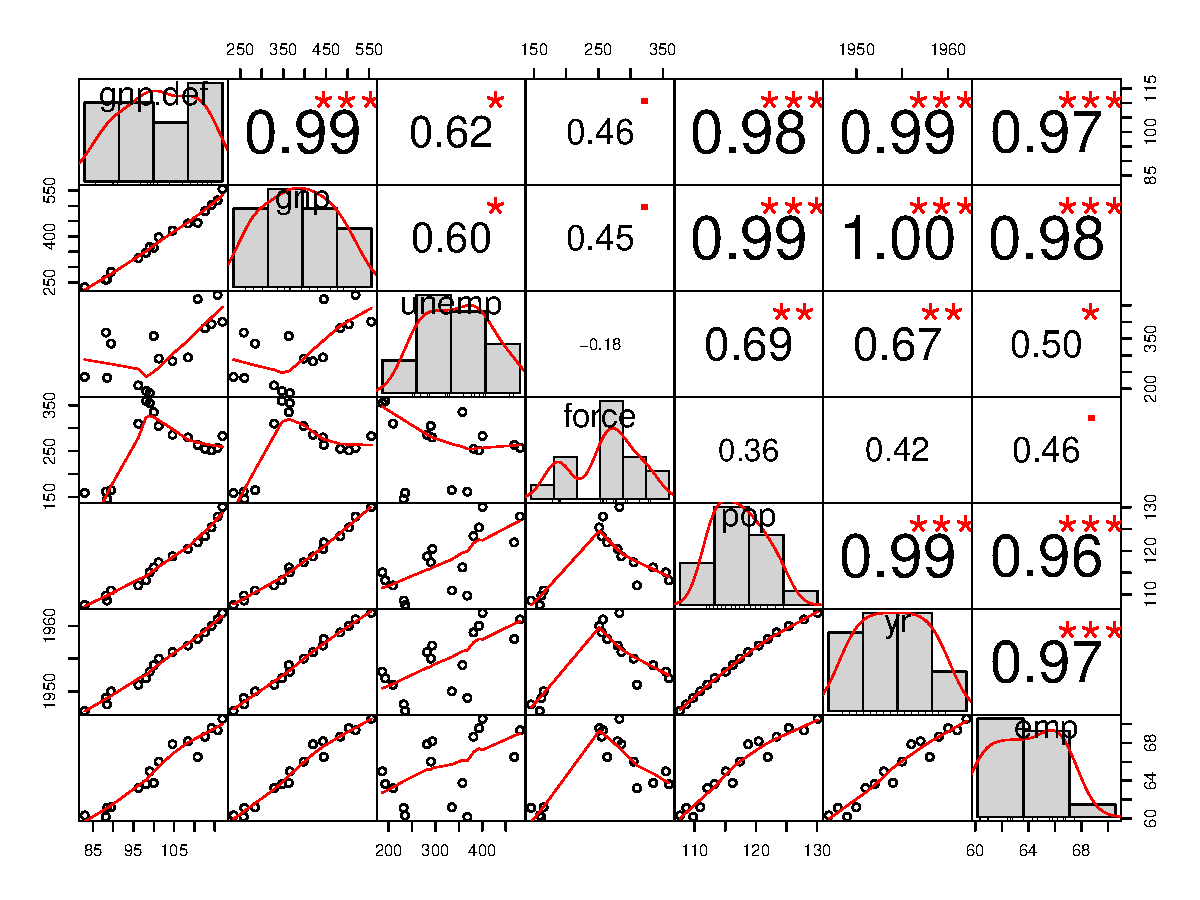
\includegraphics[width=0.5\linewidth]{figures/cormat-1} 

}

\caption{\label{fig:corrmat}Correlation Matrix}\label{fig:cormat}
\end{figure}

\begin{Shaded}
\begin{Highlighting}[]
  \CommentTok{# By far my favorite, better than other fancy stuff.}
  \CommentTok{# Perfect for continuous variables}
\end{Highlighting}
\end{Shaded}

\normalsize

\subsection{Correlation Plots (and their
arrangement)}\label{correlation-plots-and-their-arrangement}

\tiny

\begin{Shaded}
\begin{Highlighting}[]
\KeywordTok{par}\NormalTok{(}\DataTypeTok{mfrow =} \KeywordTok{c}\NormalTok{(}\DecValTok{1}\NormalTok{, }\DecValTok{2}\NormalTok{)) }\CommentTok{# 2 figures in a row}
\KeywordTok{plot}\NormalTok{(longley}\OperatorTok{$}\NormalTok{gnp, longley}\OperatorTok{$}\NormalTok{force, }\DataTypeTok{xlab =} \StringTok{"GNP"}\NormalTok{, }\DataTypeTok{ylab =} \StringTok{"Size of Armed Force"}\NormalTok{, }\DataTypeTok{main =} \StringTok{"GNP"}\NormalTok{)}
\KeywordTok{plot}\NormalTok{(}\KeywordTok{log}\NormalTok{(longley}\OperatorTok{$}\NormalTok{gnp), longley}\OperatorTok{$}\NormalTok{force, }\DataTypeTok{xlab =} \StringTok{"log(GNP)"}\NormalTok{, }\DataTypeTok{ylab =} \StringTok{"Size of Armed Force"}\NormalTok{, }
     \DataTypeTok{main =} \StringTok{"log(GNP)"}\NormalTok{)}
\end{Highlighting}
\end{Shaded}

\begin{figure}[h!]

{\centering 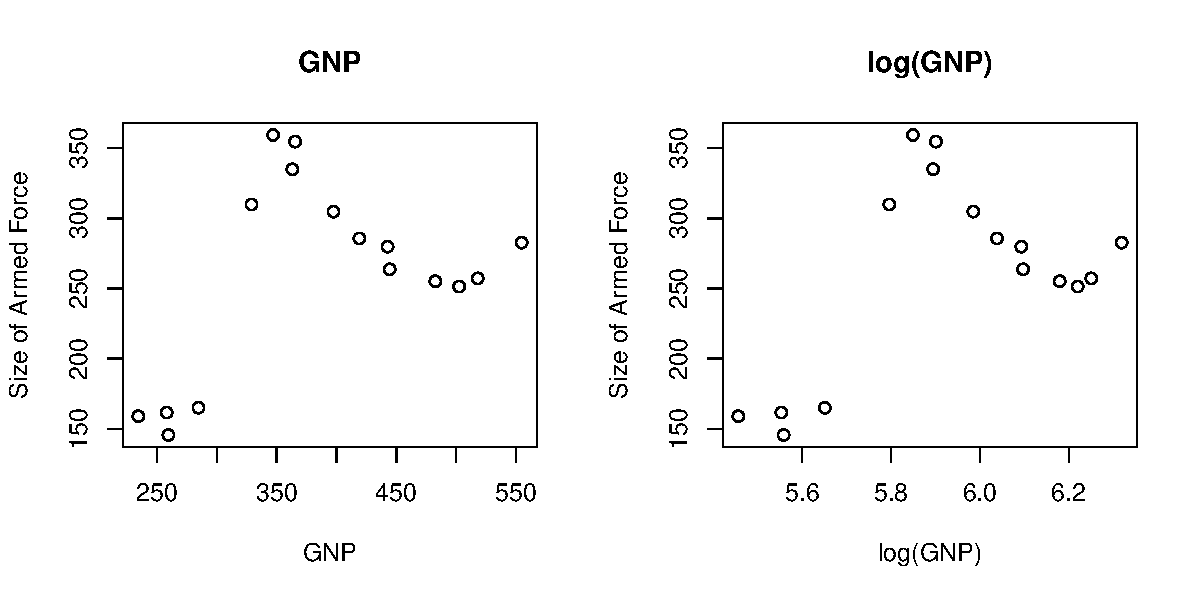
\includegraphics[width=0.9\linewidth]{figures/cor1-1} 

}

\caption{\label{fig:force-and-gnp1}Size of Armed Force and GNP (default)}\label{fig:cor1}
\end{figure}

\normalsize

\tiny

\begin{Shaded}
\begin{Highlighting}[]
\CommentTok{# The cowplot package: https://cran.r-project.org/web/packages/cowplot/vignettes/plot_grid.html}
\NormalTok{fig_cor1 <-}\StringTok{ }\KeywordTok{ggplot}\NormalTok{(longley, }\KeywordTok{aes}\NormalTok{(}\DataTypeTok{x =}\NormalTok{ gnp, }\DataTypeTok{y =}\NormalTok{ force)) }\OperatorTok{+}\StringTok{ }\KeywordTok{geom_point}\NormalTok{() }\OperatorTok{+}\StringTok{ }
\StringTok{  }\KeywordTok{geom_smooth}\NormalTok{(}\DataTypeTok{method =} \StringTok{"loess"}\NormalTok{) }\OperatorTok{+}\StringTok{ }\KeywordTok{xlab}\NormalTok{(}\StringTok{"GNP"}\NormalTok{) }\OperatorTok{+}\StringTok{ }\KeywordTok{ylab}\NormalTok{(}\StringTok{"Size of Armed Force"}\NormalTok{) }\OperatorTok{+}
\StringTok{  }\KeywordTok{ggtitle}\NormalTok{(}\StringTok{"GNP"}\NormalTok{)}
\NormalTok{fig_cor2 <-}\StringTok{ }\KeywordTok{ggplot}\NormalTok{(longley, }\KeywordTok{aes}\NormalTok{(}\DataTypeTok{x =} \KeywordTok{log}\NormalTok{(gnp), }\DataTypeTok{y =}\NormalTok{ force)) }\OperatorTok{+}\StringTok{ }\KeywordTok{geom_point}\NormalTok{() }\OperatorTok{+}\StringTok{ }
\StringTok{  }\KeywordTok{geom_smooth}\NormalTok{(}\DataTypeTok{method =} \StringTok{"loess"}\NormalTok{) }\OperatorTok{+}\StringTok{ }\KeywordTok{xlab}\NormalTok{(}\StringTok{"GNP"}\NormalTok{) }\OperatorTok{+}\StringTok{ }\KeywordTok{ylab}\NormalTok{(}\StringTok{"Size of Armed Force"}\NormalTok{) }\OperatorTok{+}
\StringTok{  }\KeywordTok{ggtitle}\NormalTok{(}\StringTok{"log(GNP)"}\NormalTok{)}
\KeywordTok{plot_grid}\NormalTok{(fig_cor1, fig_cor2, }\DataTypeTok{ncol =} \DecValTok{2}\NormalTok{)}
\end{Highlighting}
\end{Shaded}

\begin{figure}[h!]

{\centering 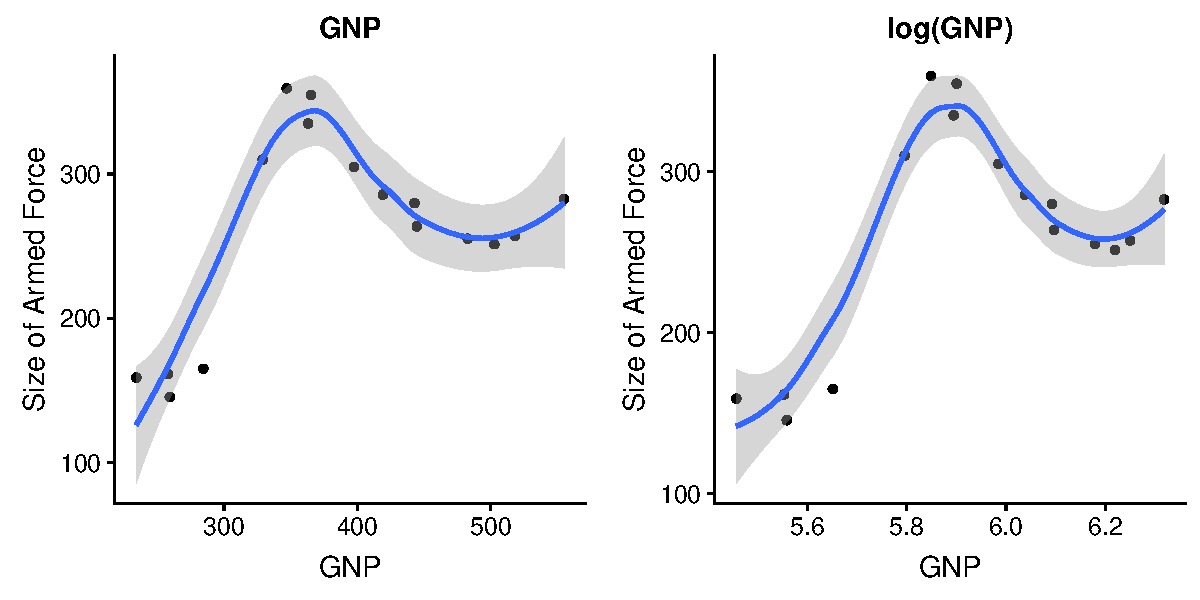
\includegraphics[width=0.9\linewidth]{figures/cor2-1} 

}

\caption{\label{fig:force-and-gnp2}Size of Armed Force and GNP (ggplot)}\label{fig:cor2}
\end{figure}

\normalsize

\clearpage

\section{Models}\label{models}

Clearly state your model and the assumption of the model.

(Alignment Style 1:)

\begin{gather*}
  \text{Model 1: } \quad \text{Armed Force}_i = \beta_0 + \beta_1 \text{Unemployment}_i + \beta_2 \text{GNP}_i + \epsilon_i \\
  \text{Model 2: } \quad \text{Armed Force}_i = \beta_0 + \beta_1 \text{Unemployment}_i + \beta_2 \text{GNP}_i + \beta_3 \text{Population}_i + \epsilon_i \\
  \text{Model 3: } \quad \text{Armed Force}_i = \beta_0 + \beta_1 \text{Unemployment}_i + \beta_2 \text{GNP}_i  + \beta_3 \text{GNP}_i^2 + \beta_4 \text{Population}_i + \epsilon_i \\
  \text{Model 4: } \quad \text{Armed Force}_i = \beta_0 + \beta_1 \text{Unemployment}_i + \beta_2 \text{GNP}_i  + \beta_3 \text{GNP}_i^2 + \beta_4 \text{Population}_i + \beta_5 \text{Year}_i + \epsilon_i \\
  \text{For all models, I assume }  \epsilon \sim N(0, \sigma^2)
\end{gather*}

(Alignment Style 2:)

\begin{align*}
  \text{Model 1: } & \text{Armed Force}_i = \beta_0 + \beta_1 \text{Unemployment}_i + \beta_2 \text{GNP}_i + \epsilon_i \\
  \text{Model 2: } & \text{Armed Force}_i = \beta_0 + \beta_1 \text{Unemployment}_i + \beta_2 \text{GNP}_i + \beta_3 \text{Population}_i + \epsilon_i \\
  \text{Model 3: } & \text{Armed Force}_i = \beta_0 + \beta_1 \text{Unemployment}_i + \beta_2 \text{GNP}_i  + \beta_3 \text{GNP}_i^2 + \beta_4 \text{Population}_i + \epsilon_i \\
  \text{Model 4: } & \text{Armed Force}_i = \beta_0 + \beta_1 \text{Unemployment}_i + \beta_2 \text{GNP}_i  + \beta_3 \text{GNP}_i^2 + \beta_4 \text{Population}_i + \beta_5 \text{Year}_i + \epsilon_i
\end{align*}\begin{equation*}
  \text{For all models, I assume } \epsilon \sim N(0, \sigma^2)
\end{equation*}

\tiny

\begin{Shaded}
\begin{Highlighting}[]
\CommentTok{#---------------------------}
\CommentTok{# Fit models}
\CommentTok{#---------------------------}
  \CommentTok{# Tips: store a group of model in a list}
  \CommentTok{# Benefits: convenient management! }
\NormalTok{  fit_models <-}\StringTok{ }\ControlFlowTok{function}\NormalTok{(d)\{}
\NormalTok{    m <-}\StringTok{ }\KeywordTok{list}\NormalTok{()}
\NormalTok{    m[[}\StringTok{"Baseline"}\NormalTok{]] <-}\StringTok{ }\KeywordTok{lm}\NormalTok{(force }\OperatorTok{~}\StringTok{ }\NormalTok{unemp }\OperatorTok{+}\StringTok{ }\NormalTok{gnp, }\DataTypeTok{data =}\NormalTok{ d)}
\NormalTok{    m[[}\StringTok{"Population"}\NormalTok{]] <-}\StringTok{ }\KeywordTok{lm}\NormalTok{(force }\OperatorTok{~}\StringTok{ }\NormalTok{unemp }\OperatorTok{+}\StringTok{ }\NormalTok{gnp }\OperatorTok{+}\StringTok{ }\NormalTok{pop, }\DataTypeTok{data =}\NormalTok{ d)}
\NormalTok{    m[[}\StringTok{"Quad Population"}\NormalTok{]] <-}\StringTok{ }\KeywordTok{lm}\NormalTok{(force }\OperatorTok{~}\StringTok{ }\NormalTok{unemp }\OperatorTok{+}\StringTok{ }\NormalTok{gnp }\OperatorTok{+}\StringTok{ }\KeywordTok{I}\NormalTok{(gnp}\OperatorTok{^}\DecValTok{2}\NormalTok{) }\OperatorTok{+}\StringTok{ }\NormalTok{pop, }\DataTypeTok{data =}\NormalTok{ d, }
                                  \DataTypeTok{family =}\NormalTok{ gaussian)}
\NormalTok{    m[[}\StringTok{"Year"}\NormalTok{]] <-}\StringTok{ }\KeywordTok{lm}\NormalTok{(force }\OperatorTok{~}\StringTok{ }\NormalTok{unemp }\OperatorTok{+}\StringTok{ }\NormalTok{gnp }\OperatorTok{+}\StringTok{ }\KeywordTok{I}\NormalTok{(gnp}\OperatorTok{^}\DecValTok{2}\NormalTok{) }\OperatorTok{+}\StringTok{ }\NormalTok{pop }\OperatorTok{+}\StringTok{ }\NormalTok{yr, }\DataTypeTok{data =}\NormalTok{ d)}
\NormalTok{    m}
\NormalTok{  \}}

\NormalTok{  m <-}\StringTok{ }\KeywordTok{fit_models}\NormalTok{(longley)}
\end{Highlighting}
\end{Shaded}

\normalsize

\clearpage

\section{Results (Tables)}\label{results-tables}

Table \ref{tab:arm1} reports all models with no labels. Table
\ref{tab:arm2} reports part of the models. Table \ref{tab:arm3} label
the variables, reset the number of digits to report etc.

\tiny

\begin{Shaded}
\begin{Highlighting}[]
\CommentTok{# Stargazer Quick Reference: https://www.jakeruss.com/cheatsheets/stargazer/}
\CommentTok{# Alternative: xtable. More flexible, but harder to code.}
    \CommentTok{# https://cran.r-project.org/web/packages/xtable/vignettes/xtableGallery.pdf}

\CommentTok{#-------------------------------------}
\CommentTok{# Show regression results with tables}
\CommentTok{#-------------------------------------}
  \CommentTok{# Print all models}
    \KeywordTok{stargazer}\NormalTok{(m, }\DataTypeTok{label =} \StringTok{"tab:arm1"}\NormalTok{, }
              \DataTypeTok{title =} 
                \StringTok{"(All Models) Economic Determinants of the Size of Armed Force"}\NormalTok{,}
              \DataTypeTok{header =} \OtherTok{FALSE}\NormalTok{, }\DataTypeTok{type =}\NormalTok{ out_type)}
\end{Highlighting}
\end{Shaded}

\begin{table}[!htbp] \centering 
  \caption{(All Models) Economic Determinants of the Size of Armed Force} 
  \label{tab:arm1} 
\begin{tabular}{@{\extracolsep{5pt}}lcccc} 
\\[-1.8ex]\hline 
\hline \\[-1.8ex] 
 & \multicolumn{4}{c}{\textit{Dependent variable:}} \\ 
\cline{2-5} 
\\[-1.8ex] & \multicolumn{4}{c}{force} \\ 
\\[-1.8ex] & (1) & (2) & (3) & (4)\\ 
\hline \\[-1.8ex] 
 unemp & $-$0.525$^{**}$ & $-$0.227 & $-$0.825$^{***}$ & $-$0.398 \\ 
  & (0.181) & (0.317) & (0.255) & (0.428) \\ 
  & & & & \\ 
 gnp & 0.611$^{***}$ & 2.448 & 2.101$^{*}$ & 7.317 \\ 
  & (0.170) & (1.628) & (1.075) & (4.377) \\ 
  & & & & \\ 
 I(gnp$\hat{\mkern6mu}$2) &  &  & $-$0.007$^{***}$ & $-$0.010$^{***}$ \\ 
  &  &  & (0.002) & (0.003) \\ 
  & & & & \\ 
 pop &  & $-$28.928 & 59.152$^{*}$ & 79.852$^{**}$ \\ 
  &  & (25.485) & (27.333) & (31.599) \\ 
  & & & & \\ 
 yr &  &  &  & $-$93.220 \\ 
  &  &  &  & (75.935) \\ 
  & & & & \\ 
 Constant & 191.458$^{***}$ & 2,780.931 & $-$6,123.924$^{**}$ & 171,987.500 \\ 
  & (56.948) & (2,281.964) & (2,648.690) & (145,108.600) \\ 
  & & & & \\ 
\hline \\[-1.8ex] 
Observations & 16 & 16 & 16 & 16 \\ 
R$^{2}$ & 0.514 & 0.561 & 0.826 & 0.848 \\ 
Adjusted R$^{2}$ & 0.440 & 0.452 & 0.762 & 0.773 \\ 
Residual Std. Error & 52.098 (df = 13) & 51.529 (df = 12) & 33.935 (df = 11) & 33.179 (df = 10) \\ 
F Statistic & 6.883$^{***}$ (df = 2; 13) & 5.120$^{**}$ (df = 3; 12) & 13.021$^{***}$ (df = 4; 11) & 11.198$^{***}$ (df = 5; 10) \\ 
\hline 
\hline \\[-1.8ex] 
\textit{Note:}  & \multicolumn{4}{r}{$^{*}$p$<$0.1; $^{**}$p$<$0.05; $^{***}$p$<$0.01} \\ 
\end{tabular} 
\end{table}

\begin{Shaded}
\begin{Highlighting}[]
      \CommentTok{# If you input a list of models, it will report them all in one table.}
      \CommentTok{# Remember to add label and title to your table. }
      \CommentTok{# A table of ambiguous meaning is not worth reporting}

  \CommentTok{# Print a subset of models}
    \KeywordTok{stargazer}\NormalTok{(m[[}\StringTok{"Baseline"}\NormalTok{]], m[[}\StringTok{"Population"}\NormalTok{]], }\DataTypeTok{label =} \StringTok{"tab:arm2"}\NormalTok{, }
              \DataTypeTok{title =} 
                \StringTok{"(Baseline and Population) Economic Determinants of the Size of Armed Force"}\NormalTok{,}
              \DataTypeTok{header =} \OtherTok{FALSE}\NormalTok{, }\DataTypeTok{type =}\NormalTok{ out_type)}
\end{Highlighting}
\end{Shaded}

\begin{table}[!htbp] \centering 
  \caption{(Baseline and Population) Economic Determinants of the Size of Armed Force} 
  \label{tab:arm2} 
\begin{tabular}{@{\extracolsep{5pt}}lcc} 
\\[-1.8ex]\hline 
\hline \\[-1.8ex] 
 & \multicolumn{2}{c}{\textit{Dependent variable:}} \\ 
\cline{2-3} 
\\[-1.8ex] & \multicolumn{2}{c}{force} \\ 
\\[-1.8ex] & (1) & (2)\\ 
\hline \\[-1.8ex] 
 unemp & $-$0.525$^{**}$ & $-$0.227 \\ 
  & (0.181) & (0.317) \\ 
  & & \\ 
 gnp & 0.611$^{***}$ & 2.448 \\ 
  & (0.170) & (1.628) \\ 
  & & \\ 
 pop &  & $-$28.928 \\ 
  &  & (25.485) \\ 
  & & \\ 
 Constant & 191.458$^{***}$ & 2,780.931 \\ 
  & (56.948) & (2,281.964) \\ 
  & & \\ 
\hline \\[-1.8ex] 
Observations & 16 & 16 \\ 
R$^{2}$ & 0.514 & 0.561 \\ 
Adjusted R$^{2}$ & 0.440 & 0.452 \\ 
Residual Std. Error & 52.098 (df = 13) & 51.529 (df = 12) \\ 
F Statistic & 6.883$^{***}$ (df = 2; 13) & 5.120$^{**}$ (df = 3; 12) \\ 
\hline 
\hline \\[-1.8ex] 
\textit{Note:}  & \multicolumn{2}{r}{$^{*}$p$<$0.1; $^{**}$p$<$0.05; $^{***}$p$<$0.01} \\ 
\end{tabular} 
\end{table}

\begin{Shaded}
\begin{Highlighting}[]
  \CommentTok{# Label your Table (Essential!!!)}
    \KeywordTok{stargazer}\NormalTok{(m, }\DataTypeTok{label =} \StringTok{"tab:arm3"}\NormalTok{,}
              \DataTypeTok{title =} \StringTok{"(Labeled) Economic Determinants of the Size of Armed Force"}\NormalTok{,}
              \DataTypeTok{covariate.labels =} \KeywordTok{c}\NormalTok{(}\StringTok{"Unemployment"}\NormalTok{, }\StringTok{"GNP"}\NormalTok{,}
                                   \StringTok{"GNP sq"}\NormalTok{, }\StringTok{"Population"}\NormalTok{, }\StringTok{"Year"}\NormalTok{),}
                \CommentTok{# Mind the order... Better Strategy is asigning meaningful var names}
                \CommentTok{# in the dataset. Will end up saving your time!}
              \DataTypeTok{dep.var.labels =} \StringTok{"Size of Armed Force"}\NormalTok{,}
              \DataTypeTok{digits =} \DecValTok{2}\NormalTok{,}
              \DataTypeTok{ci =} \OtherTok{TRUE}\NormalTok{,}
              \DataTypeTok{star.cutoffs =} \OtherTok{NA}\NormalTok{, }\CommentTok{# don't show stars}
              \DataTypeTok{notes =} \StringTok{"Source of Data: Longley (1967)"}\NormalTok{,}
              \DataTypeTok{font.size =} \StringTok{"footnotesize"}\NormalTok{, }\CommentTok{# Font size}
              \DataTypeTok{header =} \OtherTok{FALSE}\NormalTok{, }\DataTypeTok{type =}\NormalTok{ out_type}
\NormalTok{              )}
\end{Highlighting}
\end{Shaded}

\begin{table}[!htbp] \centering 
  \caption{(Labeled) Economic Determinants of the Size of Armed Force} 
  \label{tab:arm3} 
\footnotesize 
\begin{tabular}{@{\extracolsep{5pt}}lcccc} 
\\[-1.8ex]\hline 
\hline \\[-1.8ex] 
 & \multicolumn{4}{c}{\textit{Dependent variable:}} \\ 
\cline{2-5} 
\\[-1.8ex] & \multicolumn{4}{c}{Size of Armed Force} \\ 
\\[-1.8ex] & (1) & (2) & (3) & (4)\\ 
\hline \\[-1.8ex] 
 Unemployment & $-$0.52 & $-$0.23 & $-$0.82 & $-$0.40 \\ 
  & ($-$0.88, $-$0.17) & ($-$0.85, 0.39) & ($-$1.32, $-$0.32) & ($-$1.24, 0.44) \\ 
  & & & & \\ 
 GNP & 0.61 & 2.45 & 2.10 & 7.32 \\ 
  & (0.28, 0.94) & ($-$0.74, 5.64) & ($-$0.01, 4.21) & ($-$1.26, 15.89) \\ 
  & & & & \\ 
 GNP sq &  &  & $-$0.01 & $-$0.01 \\ 
  &  &  & ($-$0.01, $-$0.004) & ($-$0.02, $-$0.004) \\ 
  & & & & \\ 
 Population &  & $-$28.93 & 59.15 & 79.85 \\ 
  &  & ($-$78.88, 21.02) & (5.58, 112.72) & (17.92, 141.79) \\ 
  & & & & \\ 
 Year &  &  &  & $-$93.22 \\ 
  &  &  &  & ($-$242.05, 55.61) \\ 
  & & & & \\ 
 Constant & 191.46 & 2,780.93 & $-$6,123.92 & 171,987.50 \\ 
  & (79.84, 303.07) & ($-$1,691.64, 7,253.50) & ($-$11,315.26, $-$932.59) & ($-$112,420.10, 456,395.10) \\ 
  & & & & \\ 
\hline \\[-1.8ex] 
Observations & 16 & 16 & 16 & 16 \\ 
R$^{2}$ & 0.51 & 0.56 & 0.83 & 0.85 \\ 
Adjusted R$^{2}$ & 0.44 & 0.45 & 0.76 & 0.77 \\ 
Residual Std. Error & 52.10 (df = 13) & 51.53 (df = 12) & 33.94 (df = 11) & 33.18 (df = 10) \\ 
F Statistic & 6.88 (df = 2; 13) & 5.12 (df = 3; 12) & 13.02 (df = 4; 11) & 11.20 (df = 5; 10) \\ 
\hline 
\hline \\[-1.8ex] 
\textit{Note:}  & \multicolumn{4}{r}{NA} \\ 
 & \multicolumn{4}{r}{Source of Data: Longley (1967)} \\ 
\end{tabular} 
\end{table}

\normalsize

\clearpage

\section{Discussion}\label{discussion}

All results are summarized in Table \ref{tab:arm3}\ldots{} bla bla bla

\section{Citation}\label{citation}

\tiny

\normalsize

Two ways to cite:

\begin{itemize}
\tightlist
\item
  The LaTex way

  \begin{itemize}
  \tightlist
  \item
    Bla bla bla \citep{johnston2014ideology}.
  \item
    \citet[][p.234]{beramendi2008democracy} argue that\ldots{}
  \item
    Existing studies find evidence that bla bla bla
    \citep[see][for detailed explanation]{stegmueller2013many,bell2015explaining}\ldots{}
  \end{itemize}
\item
  The \texttt{Rmarkdown} way

  \begin{itemize}
  \tightlist
  \item
    Bla bla bla \citep{johnston2014ideology}.
  \item
    \citet{beramendi2008democracy} argue that\ldots{}
  \item
    Existing studies find evidence that bla bla bla \citep[see][ for
    details]{stegmueller2013many, bell2015explaining}
  \end{itemize}
\end{itemize}

\clearpage

\bibliography{biblio}

\clearpage

\section{Others (Analytical Graphs, Game
Trees\ldots{})}\label{others-analytical-graphs-game-trees}

\texttt{Rmarkdown} allows you to use all LaTex packages (put
\texttt{header\_includes:\ \textbackslash{}usepackage\{\}\ in\ in\ the\ header\ at\ the\ start\ of\ the\ document}).
For example, you can plot analytical graphs (functions, game trees etc.)
with the \texttt{TikZ} packages. See more examples here:\newline
\texttt{http://www.sfu.ca/\textasciitilde{}haiyunc/notes/Game\_Trees\_with\_TikZ.pdf};\newline \texttt{https://sites.google.com/site/kochiuyu/Tikz}.

\section{Appendix (Code)}\label{appendix-code}

For readability, you may suppress your code within your text, and put
them all into the appendix. You can re-use a chunk of code by calling
\texttt{ref.label=(chunck\_name)}. When you reuse a chunk, you may want
to avoid running again by setting \texttt{eval=FALSE}. Again, you can
set these up as a global option with the \texttt{knitr::opts\_chunck}
command.

\tiny

\begin{Shaded}
\begin{Highlighting}[]
\CommentTok{# Show the code in the appdx, but do not run them again.}
\NormalTok{knitr}\OperatorTok{::}\NormalTok{opts_chunk}\OperatorTok{$}\KeywordTok{set}\NormalTok{(}\DataTypeTok{echo =} \OtherTok{TRUE}\NormalTok{, }\DataTypeTok{eval =} \OtherTok{FALSE}\NormalTok{)}
\end{Highlighting}
\end{Shaded}

\normalsize

\subsection{Loading the Data}\label{loading-the-data}

\tiny

\begin{Shaded}
\begin{Highlighting}[]
\CommentTok{#-----------------------------}
\CommentTok{# load your data}
\CommentTok{#-----------------------------}
  \CommentTok{# Load your dataset of interest. }
  \CommentTok{# Below is an example economic dataset coming with R}
    \KeywordTok{data}\NormalTok{(}\StringTok{"longley"}\NormalTok{)}
      \CommentTok{# J. W. Longley (1967) An appraisal of least-squares programs from }
      \CommentTok{# the point of view of the user. }
      \CommentTok{# Journal of the American Statistical Association 62, 819-841.}
  \CommentTok{# Just to mess up the dataset by a bit}
    \KeywordTok{names}\NormalTok{(longley) <-}\StringTok{ }\KeywordTok{c}\NormalTok{(}\StringTok{"gnp.def"}\NormalTok{, }\StringTok{"gnp"}\NormalTok{, }\StringTok{"unemp"}\NormalTok{, }\StringTok{"force"}\NormalTok{, }\StringTok{"pop"}\NormalTok{, }\StringTok{"yr"}\NormalTok{, }\StringTok{"emp"}\NormalTok{)}
\end{Highlighting}
\end{Shaded}

\normalsize

\subsection{Generating a Correlation
Matrix}\label{generating-a-correlation-matrix}

\tiny

\begin{Shaded}
\begin{Highlighting}[]
\CommentTok{#---------------------------}
\CommentTok{# Correlation Matrix}
\CommentTok{#---------------------------}
\NormalTok{  PerformanceAnalytics}\OperatorTok{::}\KeywordTok{chart.Correlation}\NormalTok{(longley)}
  \CommentTok{# By far my favorite, better than other fancy stuff.}
  \CommentTok{# Perfect for continuous variables}
\end{Highlighting}
\end{Shaded}

\normalsize

\subsection{Fitting Models}\label{fitting-models}

\tiny

\begin{Shaded}
\begin{Highlighting}[]
\CommentTok{#---------------------------}
\CommentTok{# Fit models}
\CommentTok{#---------------------------}
  \CommentTok{# Tips: store a group of model in a list}
  \CommentTok{# Benefits: convenient management! }
\NormalTok{  fit_models <-}\StringTok{ }\ControlFlowTok{function}\NormalTok{(d)\{}
\NormalTok{    m <-}\StringTok{ }\KeywordTok{list}\NormalTok{()}
\NormalTok{    m[[}\StringTok{"Baseline"}\NormalTok{]] <-}\StringTok{ }\KeywordTok{lm}\NormalTok{(force }\OperatorTok{~}\StringTok{ }\NormalTok{unemp }\OperatorTok{+}\StringTok{ }\NormalTok{gnp, }\DataTypeTok{data =}\NormalTok{ d)}
\NormalTok{    m[[}\StringTok{"Population"}\NormalTok{]] <-}\StringTok{ }\KeywordTok{lm}\NormalTok{(force }\OperatorTok{~}\StringTok{ }\NormalTok{unemp }\OperatorTok{+}\StringTok{ }\NormalTok{gnp }\OperatorTok{+}\StringTok{ }\NormalTok{pop, }\DataTypeTok{data =}\NormalTok{ d)}
\NormalTok{    m[[}\StringTok{"Quad Population"}\NormalTok{]] <-}\StringTok{ }\KeywordTok{lm}\NormalTok{(force }\OperatorTok{~}\StringTok{ }\NormalTok{unemp }\OperatorTok{+}\StringTok{ }\NormalTok{gnp }\OperatorTok{+}\StringTok{ }\KeywordTok{I}\NormalTok{(gnp}\OperatorTok{^}\DecValTok{2}\NormalTok{) }\OperatorTok{+}\StringTok{ }\NormalTok{pop, }\DataTypeTok{data =}\NormalTok{ d, }
                                  \DataTypeTok{family =}\NormalTok{ gaussian)}
\NormalTok{    m[[}\StringTok{"Year"}\NormalTok{]] <-}\StringTok{ }\KeywordTok{lm}\NormalTok{(force }\OperatorTok{~}\StringTok{ }\NormalTok{unemp }\OperatorTok{+}\StringTok{ }\NormalTok{gnp }\OperatorTok{+}\StringTok{ }\KeywordTok{I}\NormalTok{(gnp}\OperatorTok{^}\DecValTok{2}\NormalTok{) }\OperatorTok{+}\StringTok{ }\NormalTok{pop }\OperatorTok{+}\StringTok{ }\NormalTok{yr, }\DataTypeTok{data =}\NormalTok{ d)}
\NormalTok{    m}
\NormalTok{  \}}

\NormalTok{  m <-}\StringTok{ }\KeywordTok{fit_models}\NormalTok{(longley)}
\end{Highlighting}
\end{Shaded}

\normalsize

\subsection{Presenting Results in
Tables}\label{presenting-results-in-tables}

\tiny

\begin{Shaded}
\begin{Highlighting}[]
\CommentTok{# Stargazer Quick Reference: https://www.jakeruss.com/cheatsheets/stargazer/}
\CommentTok{# Alternative: xtable. More flexible, but harder to code.}
    \CommentTok{# https://cran.r-project.org/web/packages/xtable/vignettes/xtableGallery.pdf}

\CommentTok{#-------------------------------------}
\CommentTok{# Show regression results with tables}
\CommentTok{#-------------------------------------}
  \CommentTok{# Print all models}
    \KeywordTok{stargazer}\NormalTok{(m, }\DataTypeTok{label =} \StringTok{"tab:arm1"}\NormalTok{, }
              \DataTypeTok{title =} 
                \StringTok{"(All Models) Economic Determinants of the Size of Armed Force"}\NormalTok{,}
              \DataTypeTok{header =} \OtherTok{FALSE}\NormalTok{, }\DataTypeTok{type =}\NormalTok{ out_type)}
      \CommentTok{# If you input a list of models, it will report them all in one table.}
      \CommentTok{# Remember to add label and title to your table. }
      \CommentTok{# A table of ambiguous meaning is not worth reporting}

  \CommentTok{# Print a subset of models}
    \KeywordTok{stargazer}\NormalTok{(m[[}\StringTok{"Baseline"}\NormalTok{]], m[[}\StringTok{"Population"}\NormalTok{]], }\DataTypeTok{label =} \StringTok{"tab:arm2"}\NormalTok{, }
              \DataTypeTok{title =} 
                \StringTok{"(Baseline and Population) Economic Determinants of the Size of Armed Force"}\NormalTok{,}
              \DataTypeTok{header =} \OtherTok{FALSE}\NormalTok{, }\DataTypeTok{type =}\NormalTok{ out_type)}

  \CommentTok{# Label your Table (Essential!!!)}
    \KeywordTok{stargazer}\NormalTok{(m, }\DataTypeTok{label =} \StringTok{"tab:arm3"}\NormalTok{,}
              \DataTypeTok{title =} \StringTok{"(Labeled) Economic Determinants of the Size of Armed Force"}\NormalTok{,}
              \DataTypeTok{covariate.labels =} \KeywordTok{c}\NormalTok{(}\StringTok{"Unemployment"}\NormalTok{, }\StringTok{"GNP"}\NormalTok{,}
                                   \StringTok{"GNP sq"}\NormalTok{, }\StringTok{"Population"}\NormalTok{, }\StringTok{"Year"}\NormalTok{),}
                \CommentTok{# Mind the order... Better Strategy is asigning meaningful var names}
                \CommentTok{# in the dataset. Will end up saving your time!}
              \DataTypeTok{dep.var.labels =} \StringTok{"Size of Armed Force"}\NormalTok{,}
              \DataTypeTok{digits =} \DecValTok{2}\NormalTok{,}
              \DataTypeTok{ci =} \OtherTok{TRUE}\NormalTok{,}
              \DataTypeTok{star.cutoffs =} \OtherTok{NA}\NormalTok{, }\CommentTok{# don't show stars}
              \DataTypeTok{notes =} \StringTok{"Source of Data: Longley (1967)"}\NormalTok{,}
              \DataTypeTok{font.size =} \StringTok{"footnotesize"}\NormalTok{, }\CommentTok{# Font size}
              \DataTypeTok{header =} \OtherTok{FALSE}\NormalTok{, }\DataTypeTok{type =}\NormalTok{ out_type}
\NormalTok{              )}
\end{Highlighting}
\end{Shaded}

\normalsize


\end{document}
